\section{Discussion and Conclusions}
	As per current literature on spectral fitting of the SSS \source, Bearda \textit{et al.} (2002) and Motch \textit{et al.} (2002) had arrived at the conclusion that its spectra cannot be reproduced by NLTE model atmospheres. %\cite{beardaChandra2002AA,motchXmmNewton2002AA}.
	Earlier, Hartmann \textit{et al.} (1999) had applied non-local thermodynamic equilibrium (NLTE) models, which included metal line opacities, to the spectrum extracted from the observations by BeppoSAX LECS of \source\ on 25--26 January 1997, %\cite{hartmann1999constraining}
	where the best fit was using a model consisting of two spectral components. But nevertheless, they obtained a reduced $\chi^2>2$. In the absence of a proper model describing the emission spectrum, it becomes impossible to derive fundamental parameters such as temperature, neutral hydrogen column density and luminosity. %\cite{motchXmmNewton2002AA}
	Hence, obtaining an acceptable fit for \source\ spectrum assumes crucial importance at this juncture.
%	\begin{itemize}
%		\item To include a detailed description of the physics behind the best fit model
%		\item To refer to the original publications containing the XSPEC model components where the physics is described
%		\begin{itemize}
%			\item For \texttt{TBabs}: Wilms et al. \url{https://iopscience.iop.org/article/10.1086/317016/pdf}
%			
%			Now \texttt{phabs}
%			\item For \texttt{ismabs}: Gatuzz et al. \url{https://iopscience.iop.org/article/10.1088/0004-637X/800/1/29/pdf}
%			\item For \texttt{edge}: \url{https://heasarc.gsfc.nasa.gov/xanadu/xspec/manual/node247.html}
%			\item For \texttt{rauch}: \url{http://astro.uni-tuebingen.de/~rauch/TMAF/TMAF.html}
%		\end{itemize}
%	\end{itemize}
	
	\subsection{Best-fit continuum model}
	The model, chosen for fitting the data from six different observations, consists of a publicly available\footnote{\url{http://astro.uni-tuebingen.de/~rauch/TMAF/TMAF.html}} NLTE (non-local thermal equilibrium) table model component computed from a grid of stellar model atmosphere fluxes for source emission, a photoelectric absorption model component\footnote{\url{https://heasarc.gsfc.nasa.gov/xanadu/xspec/manual/XSmodelPhabs.html}}, a model component for absorption by inter-stellar medium\footnote{\url{https://heasarc.gsfc.nasa.gov/xanadu/xspec/manual/node255.html}} and four model components to account for the presence of absorption edges\footnote{\url{https://heasarc.gsfc.nasa.gov/xanadu/xspec/manual/node247.html}}.
	
	The values of the fit statistic used, i.e. the reduced $\chi^2$, were all within the acceptable range of $1<\chi^2_\text{reduced}<2$, which warrants a model to be considered a good fit for the observed data. An inspection of the distribution of the residual suggests an approximately normal distribution, which can be observed in the best-fit models for all the observations, further supporting the validity of the model fit. Such a distribution of the residuals is displayed in figure \ref{fig:pn:resid-hist} for the observations of the EPIC-pn data.
	
	\begin{figure*}[!htb]
        \centering
        \begin{subfigure}[b]{0.51\textwidth}
            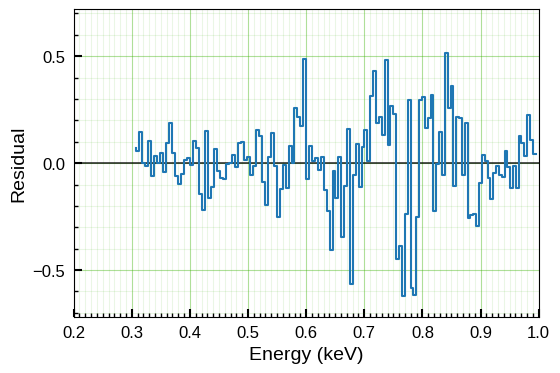
\includegraphics[width=\textwidth]{figures/resid/mr-vel-0111150101-pn_resid.png}
            \caption{Residuals between data and best-fit model for EPIC-pn observations}
            \label{fig:pn:resid}
        \end{subfigure}
        \hfill
        \begin{subfigure}[b]{0.39\textwidth}
            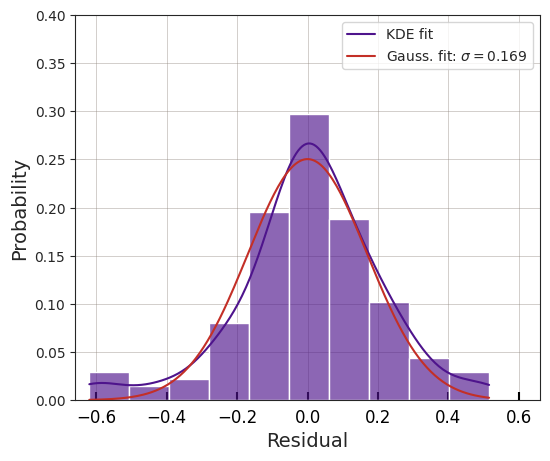
\includegraphics[width=\textwidth]{figures/resid/mr-vel-0111150101-pn_resid-hist.png}
	        \caption{Distribution of residuals from the best-fit model to EPIC-pn observations, along with the KDE function and fitted Gaussian}
	        \label{fig:pn:resid-hist}
        \end{subfigure}
        \caption{Residual statistics from best-fit model to all observations}
        \label{fig:all-obs:resid-stats}
    \end{figure*}
    
    As it can be seen in figure \ref{fig:pn:resid-hist}, the kernel density estimate (KDE) function of the distribution closely approximates a normal distribution centred about zero (with zero indicating a perfect fit) and with a standard deviation of 0.169, thereby indicating that the observed count rate data can be considered to be random fluctuations which are normally distributed about the best-fit model. Therefore, the normal distribution of the residuals indicates that they are random and do not have a systematic bias (as is expected of a good fit), thereby further validating that the model fitting performed is satisfactory for all six cases of the observations.
    
    \begin{figure}[!htb]
    	\centering
    	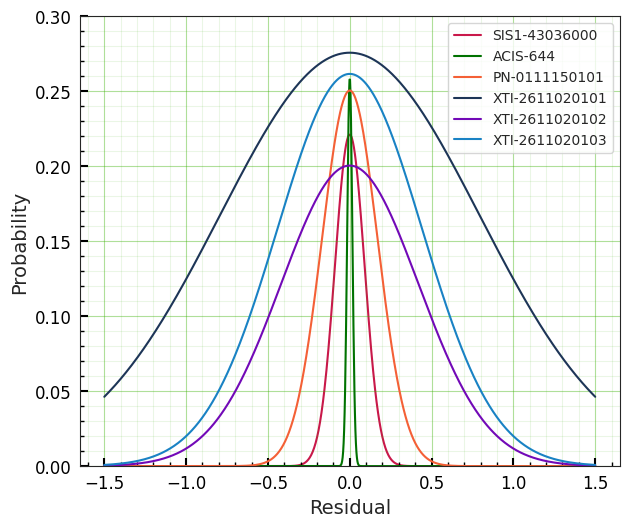
\includegraphics[width=0.45\textwidth]{figures/resid/mr-vel-resid-gaussfit_all-obs.png}
    	\caption{Gaussian approximations of the KDE functions for residual distributions of all observations}
    	\label{fig:all-obs:resid-gaussfit}
    \end{figure}
    
    In figure \ref{fig:all-obs:resid-gaussfit}, we find the Gaussian distribution fitted to all the observations. This figure shows that the quality of the fit is the best for the earlier Chandra, XMM-Newton and ASCA observations. For the recent NICER observations, the residuals show a wider spread spread about the perfect fit.
    
    %The facts that the reduced $\chi^2$ values are acceptable for a good fit and the residuals are normally distributed about zero
    
    \subsection{NLTE pure H model atmosphere}
    In a classical stellar atmosphere, which is a plane-parallel, horizontally homogenous atmosphere in hydrostatic and radiative equilibrium, a non-LTE (or NLTE) description refers to a scenario where the energy levels of some selected species may be allowed to depart from their local thermodynamic equilibrium (LTE) values \cite{hubeny2014theory}.
    	\subsubsection{Structural equations}
    	\quad\\	
	    Given below are the structural equations that are used to model an NLTE atmosphere.
	   
		In its second-order form, the \textit{radiative transfer equation} is
		\begin{align}
			\npdvt{2}{(f_\nu J_\nu)}{\tau_\nu}=J_\nu-S_\nu \label{eqn:rte-2nd-order}
		\end{align}
		where $J_\nu$ is the \textit{mean intensity} over all solid angles, $\tau_\nu$ the monochromatic \textit{optical depth}, $f_\nu$ the variable \textit{Eddington factor} and $S_\nu$ the \textit{source function}. The upper and lower boundary conditions on equation (\ref{eqn:rte-2nd-order}) are respectively
		\begin{align}
			&\left[ \pdvt{(f_\nu J_\nu)}{\tau_\nu} \right]_0=g_\nu J_\nu(0)-H_\nu^\text{ext} \label{eqn:rte-upper-bc} \\
			&\left[ \pdvt{(f_\nu J_\nu)}{\tau_\nu} \right]_{\tau_\text{max}}=H_\nu^+-\dfrac{1}{2}J_\nu \label{eqn:rte-lower-bc}
		\end{align}
		where $g_\nu$ is the \textit{surface Eddington factor}, $H_\nu^\text{ext}$, $H_\nu^+$ being the \textit{first angular moment} of specific intensity taken at the respective upper and lower boundaries of the current stellar atmospheric layer.
		
		The \textit{hydrostatic equilibrium equation} is re-cast as
		\begin{align}
			\dvt{P_\text{gas}}{m}=g-\dfrac{4\pi}{c}\integ{0}{\infty}{\dvt{K_\nu}{m}}{\nu}=g-\dfrac{4\pi}{c}\integ{0}{\infty}{\dfrac{\chi_\nu}{\rho}H_\nu}{\nu} \label{eqn:hyd-equil}
		\end{align}
		where $K_\nu$ is the \textit{second angular moment} of specific intensity, $\chi_\nu$ is the \textit{absorption coefficient} and $m$ is the \textit{Lagrangian mass}. In equation (\ref{eqn:hyd-equil}), the total pressure is composed of three parts: the \textit{gas pressure} $P_\text{gas}$, the \textit{radiation pressure} represented by the integrals on the right-hand side and the \textit{microturbulent pressure} $P_\text{turb}$ being ignored.
		
		The \textit{radiative equilibrium equation} is an expression of the conservation of total radiant flux. It may be written in an \textit{integral form} -- more accurate at upper atmospheric layer, or in a \textit{differential form} -- more accurate in deeper layers. To improve the accuracy, numerical algorithms implement a linear combination of both form as
		\begin{align}
			\alpha&\left[ \integ{0}{\infty}{(\kappa_\nu J_\nu-\eta_\nu)}{\nu} \right] \nonumber\\
				&+\beta\left[ \integ{0}{\infty}{\dvt{(f_\nu J_\nu)}{\tau_\nu}}{\nu}-\dfrac{\sigma_R}{4\pi}T_\text{eff}^4 \right]=0 \label{eqn:rad-equil}
		\end{align}
		where $\sigma_R$ is the Stefan-Boltzmann constant, $\kappa_\nu$, $\eta_\nu$ are the thermal absorption and emission coefficients respectively. In equation (\ref{eqn:rad-equil}) above, the term within the first pair of brackets contains the integral form and that within the second pair contains the differential form. The empirical coefficients $\alpha$, $\beta$ enable a transition from upper layers ($\alpha\rightarrow 1$, $\beta\rightarrow 0$) to lower layers ($\alpha\rightarrow 0$, $\beta\rightarrow 1$) -- such a transition is taken to be around the depth where the Rosseland mean optical depth is $\sim 1$.
		
		The \textit{kinetic equilibrium equations} (or \textit{rate equations}) are written for each chemical species, after having first selected those species which are to be considered to deviate from LTE. For any species, these equations may be represented by a matrix equation as
		\begin{align}
			\vsmat{A}\cdot\vsvec{n}=\vsvec{b} \label{eqn:kin-equil}
		\end{align}
		where the elements of the \textit{rate matrix} $\vsmat{A}$ are given as
		\begin{align*}
			\vmelem{A}{i}{j}&=\sum_{j\neq i}{(R_{ij}+C_{ij})} \\
			\vmelem{A}{i}{j}&=-(R_{ji}+C_{ji}),\text{ for }j\neq i\text{ and }i\neq k \\
			\vmelem{A}{k}{j}&=1+S_j
		\end{align*}
		with $k$ being the index of the \textit{characteristic level} and $R_{ij}$, $C_{ij}$ the radiative and collisional rates respectively between transition levels $i$ and $j$. It must be noted that $R_{ij}$'s implicitly involve the \textit{Saha-Boltzmann factor} $\Phi_i(T)$ which comes into play for \textit{bound-free transitions}, i.e. absorption edges
		\begin{align}
			\Phi_i(T)=\dfrac{g_i}{2g_1^+}\left( \dfrac{h^2}{2\pi m_e kT} \right)^{3/2}e^{(E_I-E_i)/kT} \label{eqn:saha-boltz-factor}
		\end{align}
		where $E_I$ is the ionization potential of the ion to which level $i$ belongs, $E_i$ the excitation energy of level $i$ and $g_1^+$ the statistical weight of the ground state of the next ion and $m_e$ the electronic mass. In equation (\ref{eqn:kin-equil}), $\vsvec{n}$ is the vector of populations of levels and the vector $\vsvec{b}$ has a single non-zero element corresponding to the characteristic level $k$ as
		\begin{align*}
			\vvelem{b}{i}=(N-n_e)\alpha_I\delta_{ki}
		\end{align*}
		where $N$ is the net populations of all levels, $n_e$ the number density of electrons and $\alpha_I$ the fractional abundance of the species $I$.
		
		The overall electrical neutrality of the medium is expressed by the \textit{charge conservation equation} as
		\begin{align}
			\sum_i{n_iZ_i}-n_e=0 \label{eqn:ch-cons}
		\end{align}
		where $Z_i$ is the charge associated with level $i$.
		
		The \textit{mass density}, which is related to the atomic level populations, can be expressed as
		\begin{align}
			\rho=(N-n_e)\mu m_H \label{eqn:mass-dens}
		\end{align}
		where $\mu$ is the mean molecular weight and $m_H$ is the mass of the H atom. A quantity known as the \textit{fictitious massive particle density} is defined as
		\begin{align}
			n_m\equiv(N-n_e)\mu \label{eqn:fict-mass-dens}
		\end{align}
		which then enables the mass density to be simply written as $\rho=n_m m_H$.
		
		The absorption coefficient included in equation (\ref{eqn:hyd-equil}) is written as the combination
		\begin{align}
			\chi_\nu=\kappa_\nu+\kappa_\nu^\text{sc} \label{eqn:abs-coeff}
		\end{align}
		where $\kappa_\nu$ is also known as the \textit{extinction coefficient} and $\kappa_\nu^\text{sc}$ the \textit{scattering coefficient}. The extinction coefficient is given as
		\begin{align}
			\kappa_\nu=\sum_{i}&\sum_{j>i}{[n_i-n_jG_{ij}(\nu)]\sigma_{ij}(\nu)} \nonumber\\
							&+\sum_{l}{n_en_l\sigma_{ll}(\nu,T)\left( 1-e^{-h\nu/kT} \right)}+\kappa_\nu^\text{addl} \label{eqn:ext-abs-coeff}
		\end{align}
		where the first term represents the contribution from \textit{bound-bound transitions} (i.e. absorption lines), the second represents that from \textit{bound-free transitions} (i.e. absorption edges) and the last term lumps together any additional opacity not written as detailed transitions. Here $G_{ij}=\frac{w_ig_i}{w_jg_j}$, with $g_i,g_j$ and $w_i,w_j$ being the respective degeneracies and statistical weights of levels $i$ and $j$ respectively. Also $\sigma_{ij}$ is the opacity of the transition between levels $i$ and $j$.
		
		The scattering coefficient in equation (\ref{eqn:abs-coeff}) is given as
		\begin{align}
			\kappa_\nu^\text{sc}=n_e\sigma_e + \sum_i{n_{\text{Ray},i}\sigma_{\text{Ray},i}} \label{eqn:sca-abs-coeff}
		\end{align}
		where $\sigma_e$, $\sigma_{\text{Ray},i}$ are the Thomson and Rayleigh scattering cross-sections respectively. For pure-hydrogen atmospheres with high temperatures, the Rayleigh scattering is negligible because the hydrogen atoms are expected to be fully ionized.
		
		In a similar manner, the \textit{total emission coefficient} is also expressed as a sum of thermal and scattering contributions as
		\begin{align}
			\eta_\nu^\text{total}=\eta_\nu+\eta_\nu^\text{sc} \label{eqn:em-coeff}
		\end{align}
		where
		\begin{align}
			\eta_\nu=\left(\dfrac{2h\nu^3}{c^2}\right)&\left[ \sum_{i}\sum_{j>i}{n_jG_{ij}(\nu)\sigma_{ij}(\nu)} \right. \nonumber\\
							&\left.+\sum_{l}{n_en_l\sigma_{ll}(\nu,T)e^{-h\nu/kT}}\right]+\eta_\nu^\text{addl} \label{eqn:ext-em-coeff}
		\end{align}
		in which, again, any additional emissivity is lumped together and given using the Planck function as $\eta_\nu^\text{addl}=\kappa_\nu^\text{addl}B_\nu$.
		
		Finally, taking into account the \textit{convective flux} $F_\text{conv}$ (if any) within the differential form of the radiative equilibrium equation (\ref{eqn:rad-equil}) as
		\begin{align}
			\integ{0}{\infty}{\dvt{(f_\nu J_\nu)}{\tau_\nu}}{\nu}+\dfrac{F_\text{conv}}{4\pi}=\dfrac{\sigma_R}{4\pi}T_\text{eff}^4 \label{eqn:rad-equil-2}
		\end{align}
		Differentiating equation (\ref{eqn:rad-equil-2}) with respect to the Lagrangian mass $m$ finally gives the \textit{radiative+convective equilibrium equation} as
		\begin{align}
			\integ{0}{\infty}{(\kappa_\nu J_\nu-\eta_\nu)}{\nu}+\dfrac{\rho}{4\pi}\dvt{F_\text{conv}}{m}=0 \label{eqn:rad-conv-equil}
		\end{align}
		
		\subsubsection{Numerical solution using ALI}
		\quad\\
		Accelerated lambda iteration (ALI) is a technique used to numerically solve the radiative transfer problem, particularly in the context of stellar atmosphere modeling \cite{hubeny2003accelerated}. It accelerates the computational process by introducing a correction term that takes into account the influence of previous iterations. A simplified procedural overview of this scheme is as follows:
		\begin{enumerate}
			\item \textit{Initial guess}: Start with an initial guess for the specific intensity of radiation at different frequencies within the atmosphere. \label{step:ali-init-guess}
			\item \textit{Lambda iteration}: Calculate how the radiation interacts with the atmosphere using the current guess for intensity, considering the absorption and emission by the species in the atmosphere. \label{step:ali-lmda-itr}
			\item \textit{Correction term}: Instead of simply accepting the result from step \ref{step:ali-lmda-itr}, ALI calculates a correction term based on the difference between the current guess and the result. \label{step:ali-corr-term}
			\item \textit{Update guess}: Add this correction term to the initial guess to obtain a new estimate for the intensity. \label{step:ali-update-guess}
			\item \textit{Iterate}: Repeat steps \ref{step:ali-lmda-itr}--\ref{step:ali-update-guess} until the solution converges, meaning the intensity values no longer change significantly between iterations. \label{step:ali-iterate}
		\end{enumerate}
		
		In order to numerically solve the structural equations for NLTE, they are first discretized over all three continuous variables: optical depth $\tau$, frequency $\nu$ and angle $\theta$. These discretized structural equations, together with a number of auxiliary relations, form a system of highly coupled, non-linear equations. Then the \textit{complete linearization scheme} \cite{auer1970non} is used to treat all equations on the same footing, thus solving all structural equations simultaneously. The T\"{u}bingen NLTE Model Atmosphere Package (TMAP)\footnote{\url{http://astro.uni-tuebingen.de/~rauch/TMAP/TMAP.html}} code uses ALI to calculate the stellar atmosphere by taking into account metal line-blanketing. With an extended grid of such atmospheres of pure-hydrogen models, synthetic spectral were calculated and these are eventually used as table models in XSPEC in the present work to simulate the source emission.
    
    \subsection{Inferences from results}
    In the current work, we are trying to understand the supersoft spectrum of \source, across observations from 1994 to 2019. The idea is to develop a robust model that explains its supersoft spectrum over different time scales and different observing instruments. The best-fit model consists of XSPEC model components which consider various factors affecting the observed spectrum:
    \begin{enumerate}[a)]
   		\item \texttt{atable\{}pure-H NLTE with $\log{g}=7$\texttt{\}}: for the actual radiation emitted by \source
   		\item \texttt{edge}: for specific wavelengths where bound-free absorption is particularly strong, leading to absorption edges
   		\item \texttt{phabs}: for describing the photoelectric absorption at the source itself.
   		\item \texttt{ismabs}: for describing how light interacts with the intervening inter-stellar medium before reaching us
   	\end{enumerate}
    	
    Initially, a simple blackbody model failed to fit the spectrum. Blackbodies emit a characteristic spectrum based on temperature, and it seems this doesn't accurately represent the complex emission from \source. Then the supersoft X-ray emission of \source\ was modelled using an NLTE stellar atmosphere model \cite{werner1999classical}. Some of these are made available as tables in appropriate FITS format to be used with the XSPEC table model component \texttt{atable} \cite{rauch2003grid,rauch2010nlte}. These models, which are essentially pre-calculated grids, vary from one another in terms of the elemental abundances, the effective temperature $T_\text{eff}$ and the effective gravity $\log{g}$ (where the gravitational acceleration $g$ is expressed in cgs units). Choosing a particular FITS file fixed the specific elemental abundance and effective gravity. Then the fitting of the model to the data is performed by using the effective temperature $T_\text{eff}$ and the redshift $z$ as parameters.
    
    During the analysis of the spectra from all six observations of \source, we found that only an NLTE model with a pure hydrogen atmosphere for which $\log{g}=7$ was able to provide a common model continuum spectrum that gave acceptable fit quality for all six observations. This model\footnote{\url{http://astro.uni-tuebingen.de/~rauch/TMAF/flux_H.html}}, developed and made publicly available by Rauch et al., has, as the core of its computational framework, the detailed representation of hydrogen atoms within stellar atmospheres. Using the TMAP,  plane-parallel, static, pure-hydrogen models were calculated, employing several simplifying assumptions to create a tractable model of the stellar atmosphere. Here, hydrogen is represented as a model atom, focussing on energy levels up to $n=14$ under NLTE conditions, neglecting the rapid depopulation of higher levels due to a compact star's strong gravity. Certain complexities like the exact treatment of light absorption are approximated for efficiency. Finally, the model only extends to a specific optical depths of
    $$\log{\tau}=-8\dots+4$$
    within the atmosphere where light can travel freely, and utilizes increased detail for calculations in specific wavelength range to ensure accuracy in that region. For the synthetic spectra, the line-broadening tables of Lemke (1997) were used \cite{lemke1997extended}.
    
    As it can be seen from table \ref{tab:res-fitting} and figure \ref{fig:L-Teff}, the effective temperature is obtained to be $\sim 10^5$ K for all six observations and luminosity is computed to be of the order of $10^{41}$ erg s$^{-1}$, which is about 3 orders of magnitude higher that what had been reported earlier by Hartmann \textit{et al.} (1999). %\cite{hartmann1999constraining}
    Such order of magnitude of $T_\text{eff}$ is also observed recently in similar fitting of CAL 83 spectrum using a pure-hydrogen NLTE model studied by Stecchini \textit{et al.} (2023). %\cite{stecchini2023revisiting}
    The high values of $T_\text{eff}$ and $L_*$ from a good fit using a pure-hydrogen model seem counterintuitive for an SSS, which is typically a white dwarf accreting from a companion star. This is because white dwarfs are usually much cooler, and the accreted material might not be pure hydrogen.
    
    However, we need to take into account the currently accepted model for SSS which is the steady nuclear burning on the surface of a white dwarf. It is likely that the companion star to \source\ is a main-sequence star, thereby hydrogen-rich. Consequently, it is possible that only hydrogen-rich matter is able to accrete around the white dwarf. This matter, upon reaching the surface of the white dwarf, owing to its large gravity, undergoes steady nuclear burning. This may explain the success of the pure-hydrogen NLTE model in fitting its spectrum. It must be borne in mind that the high $T_\text{eff}$ likely characterizes the hot accretion disk surrounding the white dwarf, and not the white dwarf itself. Friction and compression may cause the accreting matter to attain the temperatures required to undergo steady nuclear burning.
    
    There are a couple of limitations to drawing such an inference regarding \source:
    \begin{enumerate}[i.]
    	\item The NLTE model assumes a static source, which might not be entirely accurate for a dynamic system like an accretion disk.
    	\item The model assumes a pure-hydrogen composition, which might be a simplification of the actual accreting material.
    \end{enumerate}
    
    Future modeling could explore relaxing some assumptions, such as including additional elements or allowing for a dynamic disk structure. One way to do so could be by utilising the high-resolution grating spectra from observatories, such as the reflection grating spectrometer (RGS) on-board XMM-Newton, to study the absorption line profiles observed in the spectrum of \source\ and analyzing the corresponding transitions can provide valuable insights into the dynamics of the accreting material.
    
    \begin{figure*}[!htb]
    	\centering
    	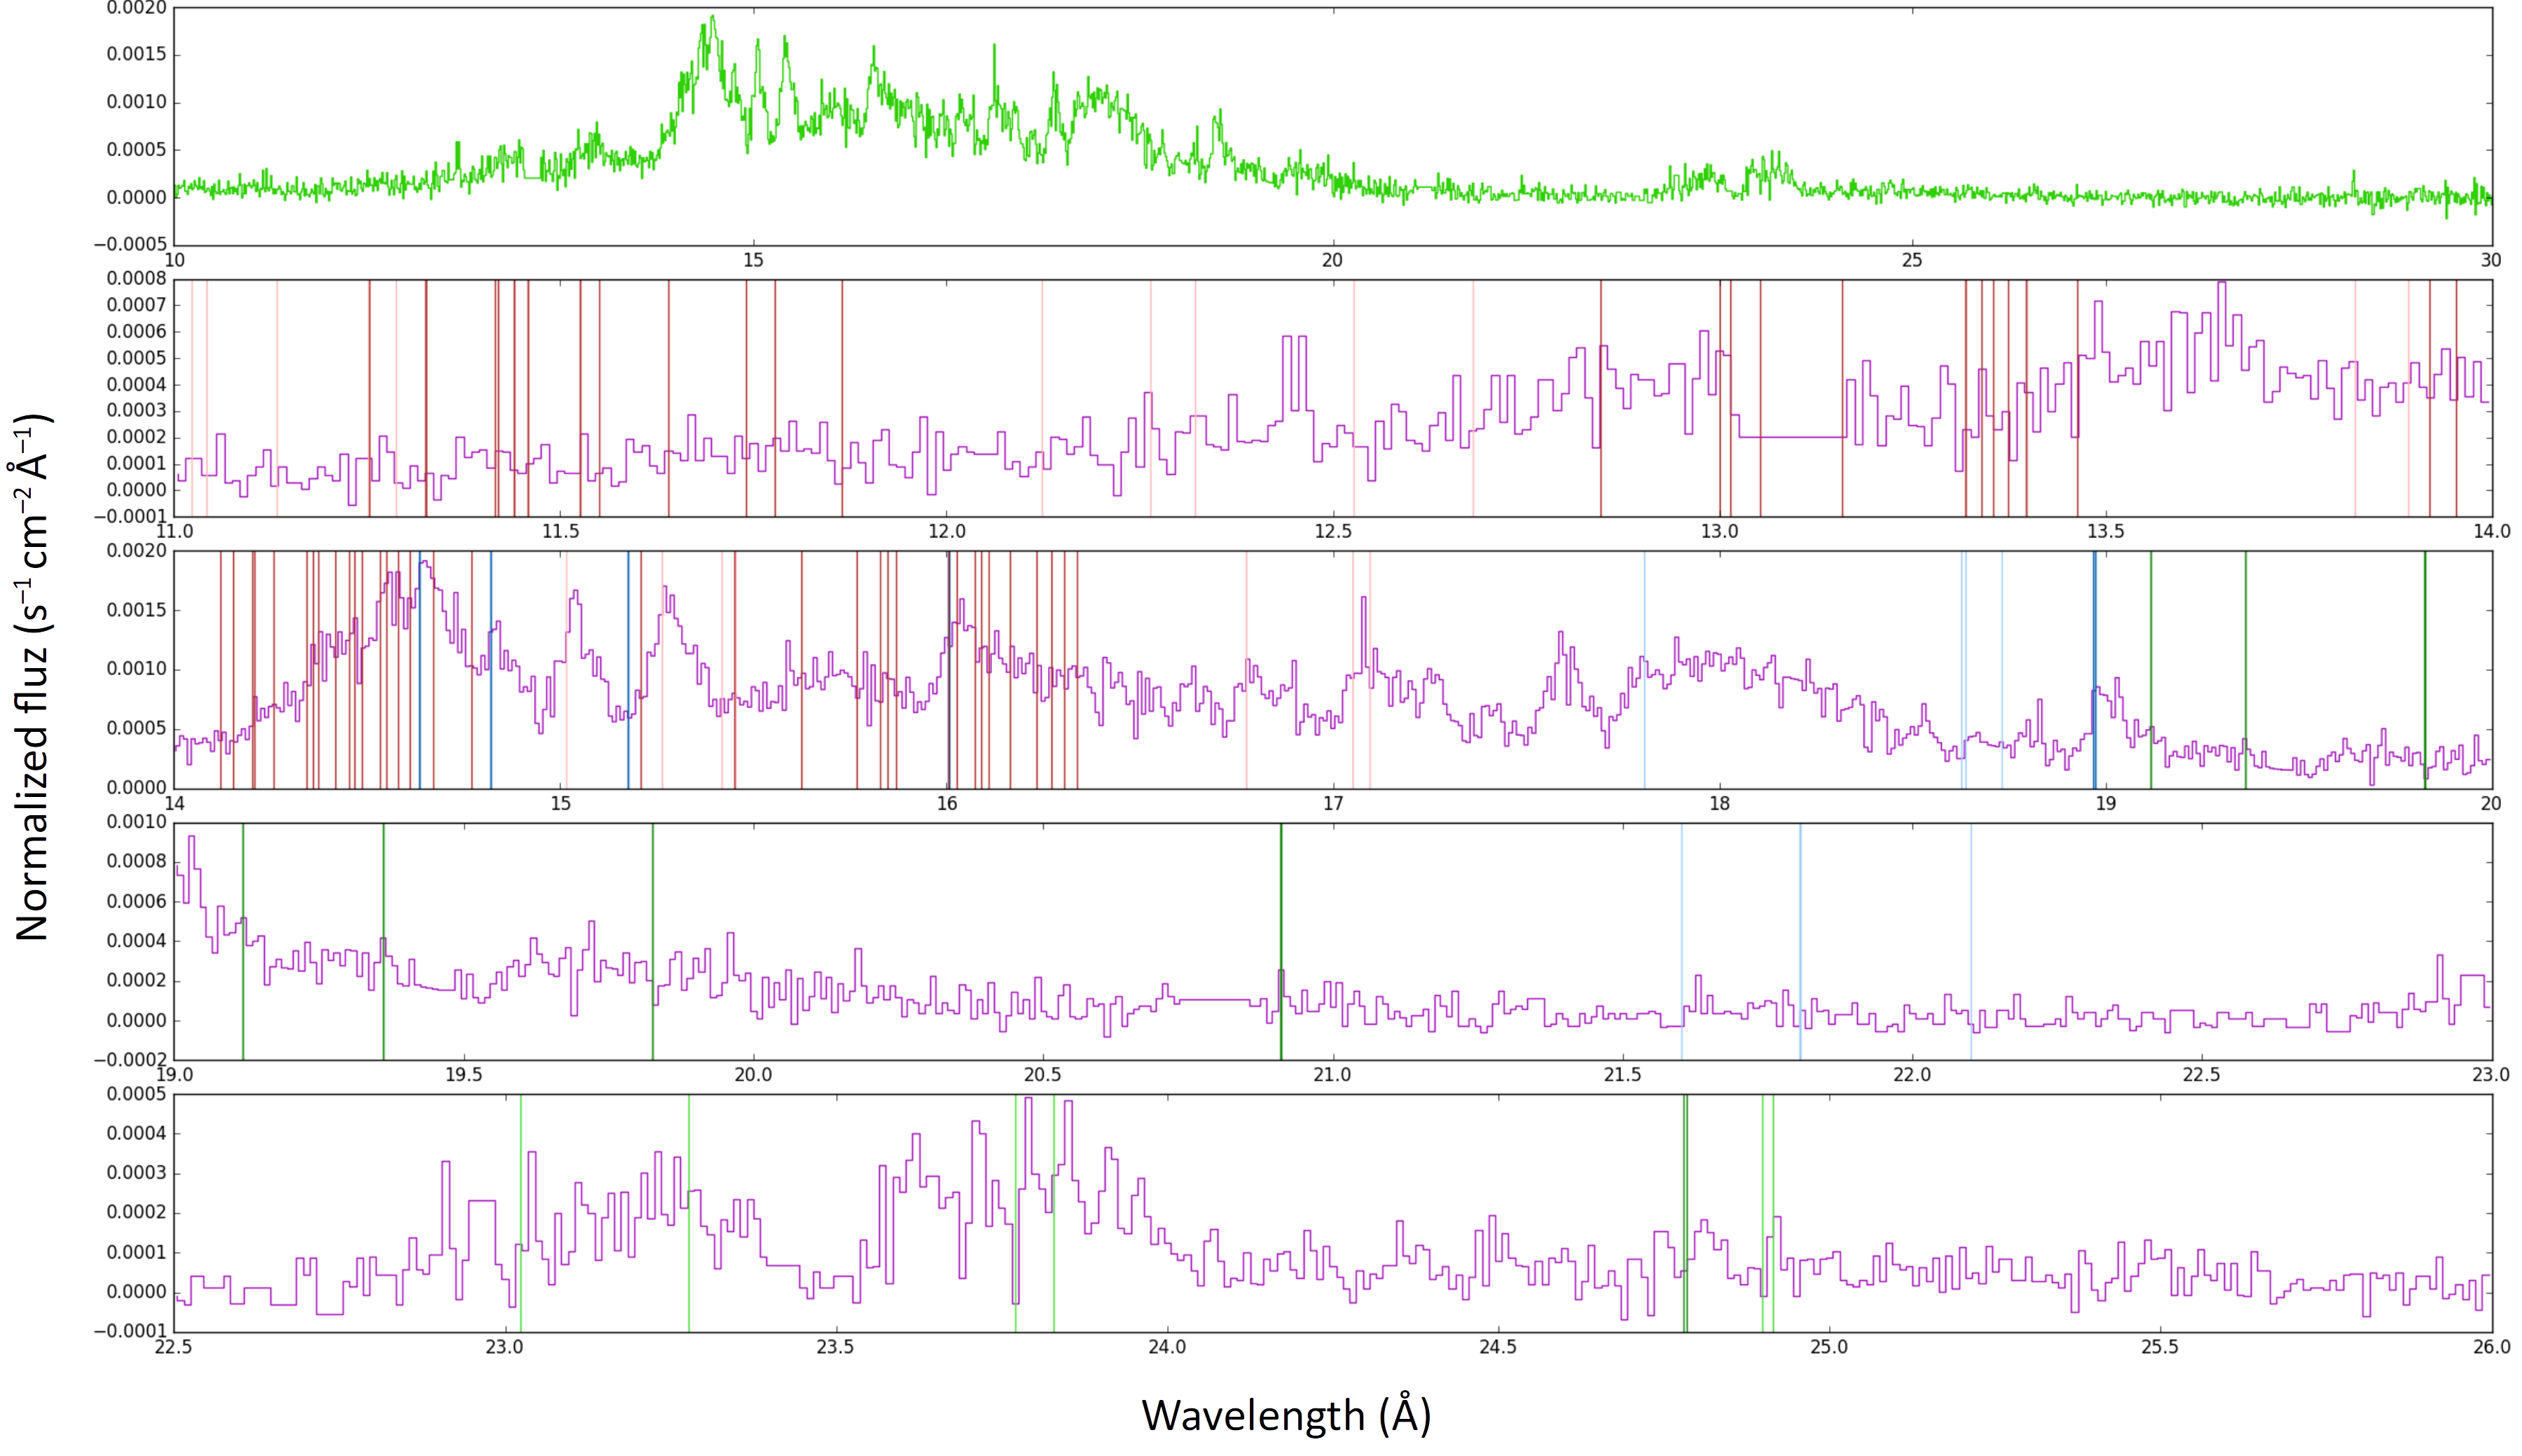
\includegraphics[width=0.9\textwidth]{figures/fig-line_identification-rgs.png}
    	\caption{Overlay of transition lines on the fluxed RGS spectrum of \source\ for Obs. ID 0111150101. The colour scheme is: N VI and N VII lines in light and dark green respectively, O VII and O VIII lines in light and dark blue respectively, Fe XVII and Fe XVIII lines in light and dark red respectively}
    	\label{fig:rgs-line-overlay}  
    \end{figure*}
    
    Absorption lines in the spectrum of \source\ arise due to the interaction of the emitted radiation with material along the line of sight. These lines exhibit diverse profiles, including shapes, widths, and shifts, which reflect the physical properties and dynamics of the absorbing material. Each absorption line corresponds to a specific transition of an atom or ion in the intervening material. Some of such lines are overlaid on the fluxed RGS spectrum of \source\ for the observation ID 0111150101, as presented in figure \ref{fig:rgs-line-overlay} \cite{bhattacharya2020python}. By identifying the atomic species and transitions associated with each absorption feature, one can gain insight into the composition and kinematics of the absorbing medium. While optical spectra have been extensively studied by categorizing them based on the presence or absence of certain spectral lines and identifying anomalies such as unusually strong or weak lines, similar approaches have been challenging to apply to X-ray spectra due to their limited spectral resolution. However, with nearly two decades of high-resolution grating spectra available from X-ray observations, it is now opportune to explore and develop methods that leverage these data to categorize and analyze X-ray spectra in more nuanced ways, such as that by Ness et al. (2013) \cite{ness2013obscuration}.
    
%The short-wavelength continuum benefits from the use of ff-cross sections from Sutherland (1998) which replace the older fit formula from Mihalas (1967). More importantly, the continuum flux depends on the treatment of the bf-transitions. Using the full formalism of Karzas & Latter (1961) raises the flux at 44 Å by 33\% compared with spectra calculated with the older Seaton formula and Gaunt factor (see Fig. 2). We find very good agreement of our results with the short-wavelength continuum of Barstow et al. (2003). Given the sensitivity of the soft X-ray fluxes to details of the calculation, we caution against the indiscriminate comparison of different versions of model spectra used over the decades in the calibration of various satellite instruments sensitive in the soft X-ray regime.
	
%Another aspect suggested to be important at soft X-ray energies is the suppression of the flux by Compton rather than Thomson scattering. Although Madej (1998), claimed a sizeable effect, Suleimanov et al. (2006) show that it is only at the 1\% level near the carbon K-edge in HZ43 A and Sirius B. Since the Compton effect deforms the model spectrum, we investigate the effect quantitatively below.
    
%Amongst the NLTE stellar atmosphere models, only
%the one with a pure hydrogen atmosphere (henceforth "pure H") and
%log g = 7 achieved a similar fit quality
%Also plotted in Figure 3 are the fit to data by two other NLTE mod-
%els: "H-Ca", that includes elements from H to Ca with abundance
%ratios as the Galactic halo and "H-Ni", with elements up to Ni and
%a particular metal enhanced abundance 14 based on nova V4743 Sgr
%(Rauch et al. 2010a,b). Even though aware that the H-Ca model
%was calculated with only approximate formulae to account for Stark
%broadening and is thus not suitable for precise spectral analysis, we
%reckon that this should not be an issue given the low energy resolu-
%tion of the spectra we are analysing. The H-Ni pre-calculated grid
%is only available for log g = 9, so we use this effective gravity for
%the H-Ca as well. While a reasonable agreement between data and
%model is obtained from bbody or pure H, neither of the two other
%NLTE models are able to fit the data, as evidenced by the residu-
%als, plotted in logarithm scale for clarity. Particularly, they notably
%underestimate the observed spectrum for energies beyond 0.45–
%0.5 keV. It can also be noticed that they demand a much larger effec-
%tive temperature – specially when compared to the pure H model –,
%likely due to the absorption caused by elements heavier than helium
%Besides previously mentioned models bbody,
%pure H and H-Ca (with halo abundances), we also show some other
%NLTE (from those publicly available) computed for different abun-
%dances: "pure He", a pure helium atmosphere model; "H-Ca", this
%time with solar abundances; and "He+CNO", a model with abundance
%ratios seen in some PG 1159 type objects (He:C:N:O = 33:50:2:15,
%e.g. Werner & Herwig 2006).
    
    \subsection{Relative strengths of absorption edges}
    Absorption edges are included in an XSPEC model using the multiplicative component named \texttt{edge}. On a continuum model, an absorption edge may be modelled as follows:
    \begin{align}
    	M(E)=\begin{cases}
    		{1;\quad E\leqslant E_\text{th}} \\
    		{\exp{\left[ -D\left(\dfrac{E}{E_\text{th}}\right)^{-3} \right]};\quad E> E_\text{th}}
    	\end{cases} \label{eqn:edge-comp}
    \end{align}
    In equation (\ref{eqn:edge-comp}), $E_\text{th}$ is the \textit{threshold energy} and $D$ is the \textit{absorption depth}. The model component is implemented with these two quantities being its parameters. The relative values of the absorption depths enables a comparison of the strengths of the absorption edges.
    
    The absorption depths calculated from the unfolded spectra, after obtaining the best fit to the model, are presented in table \ref{tab:abs-depth}. In all six observations, the same absorption edges were identified. For the observations made by ASCA, Chandra and XMM-Newton, the identified edges show the same trend with respect to the relative strengths of the absorption depths of these edges, i.e. the N $K$ absorption edge is the strongest, followed by the O $K$ edge, the Fe $L_3$ edge and the Ne $K$ edge with similar strengths.
    
    However, this is not the case for the three NICER observations, each of which show different edges to be the strongest. The reasons for such an inconsistency might range from instrumental effects (such as variations in the detector response with time, or changes in the gain calibration between observations) to issues with data reduction (such as inconsistencies in background subtraction, or inaccuracies in deadtime correction). Because NICER is a relatively new mission, it is a worthwhile exercise to investigate this particular inconsistency in absorption depth strength, which would include a detailed review of the NICER calibration documents, analysis of data from different detector regions, comparison with published data on similar sources and submission of relevant science proposals for new observations.